\chapter{Printed Circuit Board}
\label{cha:pcb}

In this chapter, the triangle-feed prototype from Chapter~\ref{cha:prototypes} is moved from a simplified ground plane PCB to a PCB with a WiSpry WS1040 tuner for each antenna. Apart from this, the minimized design from Chapter~\ref{cha_intro_5mm} will be elaborated and measured.

On the board, each tuner has four capacitors where each has a range from approximately \SI{0.3}{pF} to \SI{3.0}{pF}. In the matching network for the top antenna, the two first capacitors have two capacitors in parallel making the range approximately \SI{0.6}{pF} to \SI{6.0}{pF}. The tuner for the side antenna has all four capacitors connected in parallel making the range approximately \SI{1.2}{pF} to \SI{12}{pF}. The two first capacitors are tuned simultaneously (``tracking''). The side antenna then has an additional two individual capacitors for extending its tunable range while not affecting the top antenna.

The PCB used in this chapter is shown in Figure~\ref{fig:samanthas_board}.

\begin{figure}[htbp]
    \centering
    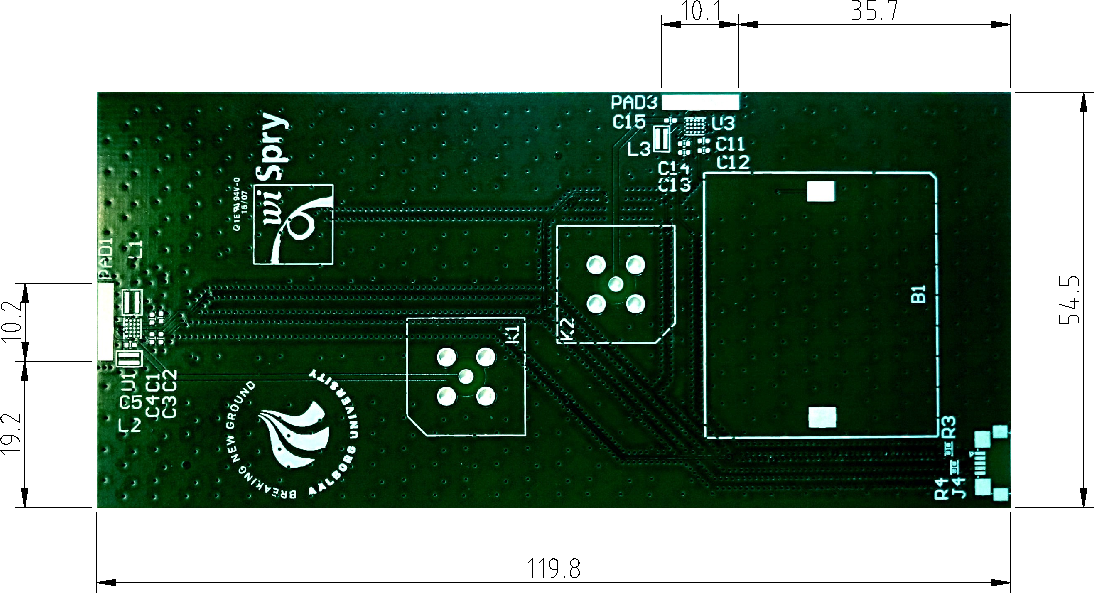
\includegraphics[scale=0.5]{img/tech_sol/samanthas_board.pdf}
    \caption{PCB used for measurements.}
    \label{fig:samanthas_board}
\end{figure}
